\documentclass[UTF8, 12pt]{ctexart}
% UTF8编码,ctexart现实中文
\usepackage{color}
% 使用颜色
\definecolor{orange}{RGB}{255,127,0}  
\definecolor{violet}{RGB}{192,0,255}  
\definecolor{aqua}{RGB}{0,255,255} 
\usepackage{geometry}
\setcounter{tocdepth}{4}
\setcounter{secnumdepth}{4}
% 设置四级目录与标题
\geometry{papersize={21cm,29.7cm}}
% 默认大小为A4
\geometry{left=3.18cm,right=3.18cm,top=2.54cm,bottom=2.54cm}
% 默认页边距为1英尺与1.25英尺
\usepackage{indentfirst}
\setlength{\parindent}{2.45em}
% 首行缩进2个中文字符
\usepackage{setspace}
\renewcommand{\baselinestretch}{1.5}
% 1.5倍行距
\usepackage{amssymb}
% 因为所以
\usepackage{amsmath}
% 数学公式
\usepackage[colorlinks,linkcolor=black,urlcolor=blue]{hyperref}
% 超链接
\usepackage{tikz}
% 绘图
\usepackage{multirow}
% 合并单元格
\newcommand{\tabincell}[2]{
\begin{tabular}{@{}#1@{}}#2\end{tabular}
}
% 空格内换行
\usepackage{graphicx}
% 缩小表格
\author{Didnelpsun}
\title{标题}
\date{}
\begin{document}
\maketitle
\pagestyle{empty}
\thispagestyle{empty}
\tableofcontents
\thispagestyle{empty}
\newpage
\pagestyle{plain}
\setcounter{page}{1}
\section{总体与样本}

\subsection{总体定义}

\textcolor{violet}{\textbf{定义:}}研究对象的全体称为\textbf{总体},组成总体的每一个元素称为\textbf{个体}。

\subsection{样本}

\subsubsection{定义}

\textcolor{violet}{\textbf{定义:}}$n$个相互独立且域总体$X$有相同概率分布的随机变量$X_1,X_2,\cdots,X_n$所组成的整体$(X_1,X_2,\cdots,X_n)$称为来自总体$X$,容量为$n$个一个\textbf{简单随机样本},简称\textbf{样本}。一次抽样结果的$n$个具体值$(x_1,x_2,\cdots,x_n)$称为来自样本$X_1,X_2,\cdots,X_n$的一个\textbf{观测值}或\textbf{样本值}。

在概率论中称为独立同分布,而在数理统计就称为简单随机样本。

\subsubsection{分布}

对于容量为$n$的样本$X_1,X_2,\cdots,X_n$有如下定理:假设总体$X$的分布函数为$F(x)$(概率密度为$f(x)$,或概率分布为$p_i=P\{X=x_i\}$),则$(X_1,X_2,\cdots,X_n)$的分布函数为$F(x_1,x_2,\cdots,x_n)=\prod\limits_{i=1}^nF(x_i)$。

对于离散型随机变量联合分布:$F(X_1=x_1,X_2=x_2,\cdots,X_n=x_n)=\prod\limits_{i=1}^nP\{X_i=x_i\}$。

对于连续型随机变量联合概率密度:$f(x_1,x_2,\cdots,x_n)=\prod\limits_{i=1}^nf(x_i)$。

\section{统计量与分布}

\subsection{统计量}

设$X_1,X_2,\cdots,X_n$来自总体$X$的一个样本,$g(x_1,x_2,\cdots,x_n)$为$n$元函数,若$g$中不含有任何未知参数,则称$g(X_1,X_2,\cdots,X_n)$为样本$X_1,X_2,\cdots,X_n$的一个\textbf{统计量}。若$(x_1,x_2,\cdots,x_n)$为样本值,则称$g(x_1,x_2,\cdots,x_n)$为$g(X_1,X_2,\cdots,X_n)$的\textbf{观测值}。

\subsection{常用统计量}

\begin{itemize}
    \item 样本均值:$\overline{X}=\dfrac{1}{n}\sum\limits_{i=1}^nX_i$。
    \item 样本方差:$S^2=\dfrac{1}{n-1}\sum\limits_{i=1}^n(X_i-\overline{X})^2$。
    \item 样本标准差:$S=\sqrt{\dfrac{1}{n-1}\sum\limits_{i=1}^n(X_i-\overline{X})^2}$。
    \item 样本$k$阶(原点)矩:$A_k=\dfrac{1}{n}\sum\limits_{i=1}^nX_i^k$($k=1,2,\cdots$)。
    \item 样本$k$中心矩:$B_k=\dfrac{1}{n}\sum\limits_{i=1}^n(X_i-\overline{X})^k$($k=1,2,\cdots$)。
\end{itemize}

\subsection{顺序统计量}

\subsubsection{概念}

将样本$X_1,X_2,\cdots,X_n$的$n$个观测量按其值从小到大的顺序排列,得到$X_{(1)}\leqslant X_{(2)}\leqslant\cdots\leqslant X_{(n)}$。

随机变量$X_{(k)}$($k=1,2,\cdots,n$)称为\textbf{第$k$顺序统计量},其中$X_{(1)}$是最小顺序统计量,而$X_{(n)}$是最大顺序统计量。

$X_{(n)}$的分布函数为$F_{(n)}(x)=[F(x)]^n$,概率密度为$f_{(n)}(x)=n[F(x)]^{n-1}f(x)$。

证明:$F_{(n)}(x)=P\{X_{(n)}\leqslant x\}=P\{\max\{x_1,\cdots,x_n\}\leqslant x\}=P\{x_1\leqslant x,\cdots,x_n\leqslant x\}=P\{x_1\leqslant x\}\cdots P\{x_n\leqslant x\}=F_{(1)}(x)\cdots F_{(n)}(x)=[F(x)]^n$。

$X_{(1)}$的分布函数为$F_{(1)}(x)=1-[1-F(x)]^n$,概率密度为$f_{(1)}(x)=n[1-F(x)]^{n-1}f(x)$。

证明:$F_{(1)}(x)=P\{X_{(1)}\leqslant x\}=P\{\min\{x_1,\cdots,x_n\}\leqslant x\}=1-P\{\min\{x_1,\cdots$\\$,x_n\}>x\}=1-P\{x_1>x,\cdots,x_n>x\}=1-P\{x_1>x\}\cdots P\{x_n>x\}=1-[1-P\{x_1\leqslant x\}]\cdots[1-P\{x_n\leqslant x\}]=1-[1-F_{(1)}(x)]\cdots[1-F_{(n)}(x)]=1-[1-F(x)]^n$。

\subsubsection{性质}

设总体$X$的期望$EX=\mu$,方差$DX=\sigma^2$,样本$X_1,X_2,\cdots,X_n$取自$X$,$\overline{X}$和$S^2$分别为样本的均值和方差,则:

\begin{itemize}
    \item $EX_i=\mu$。
    \item $DX_i=\sigma^2$。
    \item $E\overline{X}=EX=\mu$。
    \item $D\overline{X}=D\left(\dfrac{1}{n}\sum\limits_{i=1}^nx_i\right)=\dfrac{1}{n^2}n\sigma^2=\dfrac{1}{n}DX=\dfrac{\sigma^2}{n}$。
    \item $E(S^2)=E\left(\dfrac{1}{n-1}\sum\limits_{i=1}^n(x_i-\overline{x})^2\right)=E\left(\dfrac{1}{n-1}\sum\limits_{i=1}^n(x_i^2-2x_i\overline{x}+\overline{x}^2)\right)=$\\$E\left(\dfrac{1}{n-1}\left(\sum\limits_{i=1}^nx_i^2-2\overline{x}\cdot\sum\limits_{i=1}^nx_i+n\overline{x}^2\right)\right)=E\left(\dfrac{1}{n-1}\left(\sum\limits_{i=1}^nx_i^2-n\overline{x}^2\right)\right)=$\\$\dfrac{1}{n-1}E\left(\sum\limits_{i=1}^nx_i^2-n\overline{x}^2\right)=\dfrac{1}{n-1}\left(\sum\limits_{i=1}^nEx_i^2-nE\overline{x}^2\right)=\dfrac{n}{n-1}[(Ex_i)^2+Dx_i-(E\overline{x})^2-D\overline{x}]=\dfrac{n}{n-1}\left(\mu^2+\sigma^2-\mu^2-\dfrac{\sigma^2}{n}\right)=DX=\sigma^2$。
\end{itemize}

\subsection{三大分布}

\subsubsection{\texorpdfstring{$\chi^2$分布}{}}

\paragraph{概念} \leavevmode \medskip

\textcolor{violet}{\textbf{定义:}}若随机变量$X_1,X_2,\cdots,X_n$相互独立,且都服从标准正态分布,则随机变量$X=\sum\limits_{i=1}^nX_i^2$服从自由度为$n$的$\chi^2$分布,记为$X\sim\chi^2(n)$,特别地$X_i^2\sim\chi^2(1)$。

对给定的$\alpha$($0<\alpha<1$)称满足$P\{\chi^2>\chi_\alpha^2(n)\}=\int_{\chi_\alpha^2(n)}^{+\infty}f(x)\,\textrm{d}x=\alpha$的$\chi_\alpha^2(n)$为$\chi^2(n)$分布的\textbf{上$\alpha$分位点}。

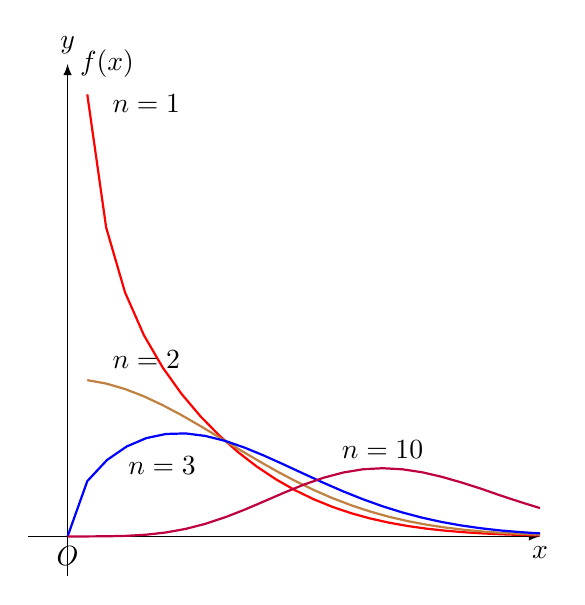
\begin{tikzpicture}[scale=2]
    \draw[-latex](-0.25,0) -- (3,0) node[below]{$x$};
    \draw[-latex](0,-0.25) -- (0,3) node[above]{$y$};
    \filldraw[black] (0,0) node[below]{$O$};
    \draw[red, thick, domain=0.125:3] plot (\x,{pow(\x,-0.5)*pow(e,-\x*\x/2)});
    \filldraw[black] (0.5,2.75) node{$n=1$};
    \draw[brown, thick, domain=0.125:3] plot (\x,{pow(e,-\x*\x/2)});
    \filldraw[black] (0.5,1.125) node{$n=2$};
    \draw[blue, thick, domain=0:3] plot (\x,{pow(\x,0.5)*pow(e,-\x*\x/2)});
    \filldraw[black] (0.6,0.45) node{$n=3$};
    \draw[purple, thick, domain=0:3] plot (\x,{pow(\x,4)*pow(e,-\x*\x/2)/5});
    \filldraw[black] (2,0.55) node{$n=10$};
    \filldraw[black] (0.25,3) node{$f(x)$};
\end{tikzpicture}
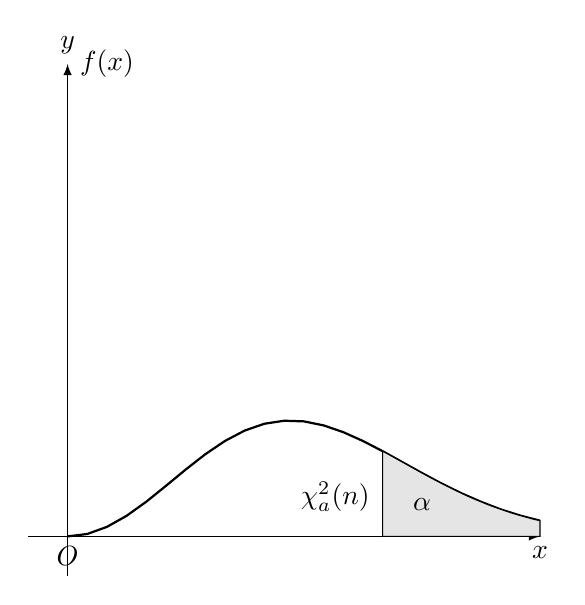
\begin{tikzpicture}[scale=2]
    \draw[-latex](-0.25,0) -- (3,0) node[below]{$x$};
    \draw[-latex](0,-0.25) -- (0,3) node[above]{$y$};
    \filldraw[black] (0,0) node[below]{$O$};
    \draw[black, thick, domain=0:3] plot (\x,{pow(\x,2)*pow(e,-\x*\x/2)});
    \filldraw[black] (1.7,0.25) node{$\chi_a^2(n)$};
    \filldraw [fill=gray!20] (2,0) -- (2,0.5) --  plot [domain=2:3,smooth] (\x,{pow(\x,2)*pow(e,-\x*\x/2)}) -- (3,0) -- (2,0);
    \filldraw[black] (0.25,3) node{$f(x)$};
    \filldraw[black] (2.25,0.2) node{$\alpha$};
\end{tikzpicture}

\paragraph{性质} \leavevmode \medskip 

\begin{itemize}
    \item 若$X_1\sim\chi^2(n_1)$,$X_2\sim\chi^2(n_2)$,$X_1X_2$相互独立,则$X_1+X_2\sim\chi^2(n_1+n_2)$。一般,若$X_i\sim\chi^2(n_i)$($i=1,2,\cdots,m$),$X_1,X_2,\cdots,X_m$相互独立,则$\sum\limits_{i=1}^mX_i\sim\chi^2\left(\sum\limits_{i=1}^mn_i\right)$。
    \item 若$X\sim\chi^2(n)$,则$EX=n$,$DX=2n$。
\end{itemize}

\subsubsection{\texorpdfstring{$t$分布}{}}

\paragraph{概念} \leavevmode \medskip

也称为学生分布。

若随机变量$X\sim N(0,1)$,$Y\sim\chi^2(n)$,$XY$相互独立,则随机变量$t=\dfrac{X}{\sqrt{Y/n}}$服从自由度为$n$的$t$分布,记为$t\sim t(n)$。

当$t\to\infty$时,$t$分布就是标准正态分布。其是偶函数,所以$Et=0$。

t分布用于根据小样本来估计呈正态分布且方差未知的总体的均值。

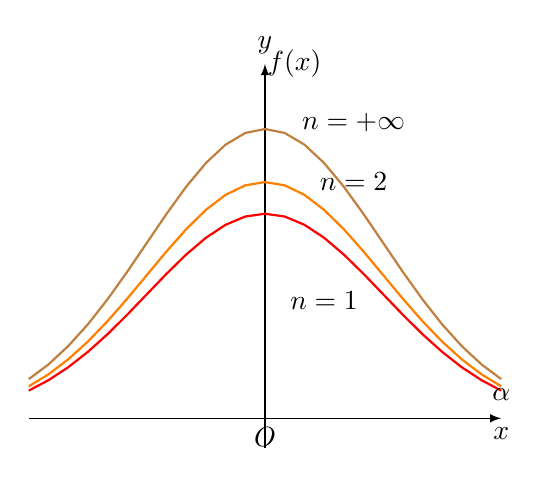
\begin{tikzpicture}[scale=1.5]
    \draw[-latex](-2,0) -- (2,0) node[below]{$x$};
    \draw[-latex](0,-0.25) -- (0,3) node[above]{$y$};
    \filldraw[black] (0,0) node[below]{$O$};
    \draw[brown, thick, domain=-2:2] plot (\x,{pow(e,-\x*\x/2)/pow(6, -0.5)});
    \filldraw[black] (0.75,2.5) node{$n=+\infty$};
    \draw[orange, thick, domain=-2:2] plot (\x,{pow(e,-\x*\x/2)/pow(4, -0.5)});
    \filldraw[black] (0.75,2) node{$n=2$};
    \draw[red, thick, domain=-2:2] plot (\x,{pow(e,-\x*\x/2)/pow(3, -0.5)});
    \filldraw[black] (0.5,1) node{$n=1$};
    \filldraw[black] (0.25,3) node{$f(x)$};
    \filldraw[black] (2,0.2) node{$\alpha$};
\end{tikzpicture}

\paragraph{性质} \leavevmode \medskip

由$t$分布的概率密度$f(x)$图形的对称性可知$P\{t>-t_\alpha(n)\}=P\{t>t_{1-\alpha}(n)\}$,所以$t_{1-\alpha}(n)=-t_\alpha(n)$。

\subsubsection{\texorpdfstring{$F$分布}{}}

\paragraph{概念} \leavevmode \medskip

若随机变量$X\sim\chi^2(n_1)$,$Y\sim\chi^2(n_2)$,且$X$与$Y$相互独立,则$F=\dfrac{X/n_1}{Y/n_2}$服从自由度为$(n_1,n_2)$的$F$分布,记为$F\sim F(n_1,n_2)$,其中$n_1$为第一自由度,$n_2$为第二自由度。

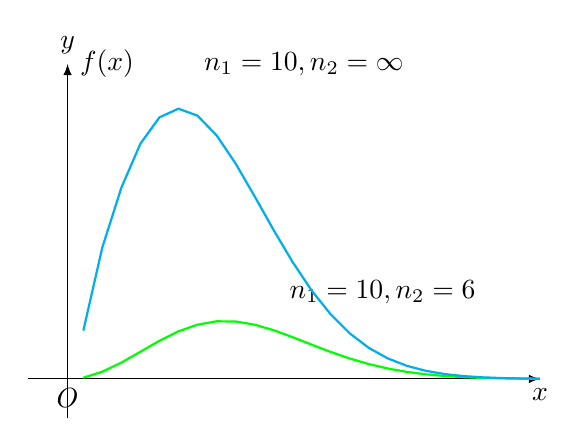
\begin{tikzpicture}[scale=2]
    \draw[-latex](-0.25,0) -- (3,0) node[below]{$x$};
    \draw[-latex](0,-0.25) -- (0,2) node[above]{$y$};
    \filldraw[black] (0,0) node[below]{$O$};
    \draw[green, thick, domain=0.1:3] plot (\x,{pow(\x,4)*pow(e,-\x*\x/2)/pow(\x,2)*pow(e,-\x*\x/2)});
    \filldraw[black] (2,0.55) node{$n_1=10,n_2=6$};
    \draw[cyan, thick, domain=0.1:3] plot (\x,{pow(\x,4)*pow(e,-\x*\x/2)/pow(\x,3)*pow(e,-\x*\x/2)*4});
    \filldraw[black] (1.5,2) node{$n_1=10,n_2=\infty$};
    \filldraw[black] (0.25,2) node{$f(x)$};
\end{tikzpicture}

\paragraph{性质} \leavevmode \medskip

\begin{itemize}
    \item 若$F\sim F(n_1,n_2)$,则$\dfrac{1}{F}\sim F(n_2,n_1)$。
    \item $F_{1-\alpha}(n_1,n_2)=\dfrac{1}{F_\alpha}(n_2,n_1)$。
\end{itemize}

证明性质二:记$F\sim F(n_2,n_1)$。

$\therefore P\{F>F_\alpha(n_2,n_1)\}=\alpha$,$P\{F\leqslant F_\alpha(n_2,n_1)\}=1-\alpha$。

取倒数:$P\left\{\dfrac{1}{F}\geqslant\dfrac{1}{F_\alpha(n_2,n_1)}\right\}=1-\alpha$。

又根据性质1:$\dfrac{1}{F}\sim F(n_1,n_2)$,$P\{\dfrac{1}{F}\geqslant F_{1-\alpha}(n_1,n_2)\}=1-\alpha$。

即$F_{1-\alpha}(n_1,n_2)=\dfrac{1}{F_\alpha}(n_2,n_1)$。

\subsection{正态总体下结论}

设$X_1,X_2,\cdots,X_n$是来自正态总体$N(\mu,\sigma^2)$的一个样本,$\overline{X}=\sum\limits_{i=1}^nX_i$,$S^2=\dfrac{1}{n-1}\sum\limits_{i=1}^n(X_i-\overline{X})^2$分别是样本的均值和方差,则:

\begin{enumerate}
    \item $\overline{X}\sim N\left(\mu,\dfrac{\sigma^2}{n}\right)$,即$\dfrac{\overline{X}-\mu}{\sigma/\sqrt{n}}=\dfrac{\sqrt{n}(\overline{X}-\mu)}{\sigma}\sim N(0,1)$。
    \item $\dfrac{1}{\sigma^2}\sum\limits_{i=1}^n(X_i-\mu)^2\sim\chi^2(n)$。
    \item $\dfrac{(n-1)S^2}{\sigma^2}=\sum\limits_{i=1}^n\left(\dfrac{X_i-\overline{X}}{\sigma}\right)^2\sim\chi^2(n-1)$($\mu$未知时,在2中用$\overline{X}$代替$\mu$)。
    \item $\overline{X}$与$S^2$相互独立,$\dfrac{\sqrt{n}(\overline{X}-\mu)}{S}\sim t(n-1)$($\sigma$未知时在1中用$S$代替$\sigma$)。进一步有$\dfrac{n(\overline{X}-\mu)^2}{S^2}\sim F(1,n-1)$。
\end{enumerate}

设$X_1,X_2,\cdots,X_m$是来自正态总体$N(\mu_1,\sigma_1^2)$的一个样本,设$Y_1,Y_2,\cdots,Y_n$是来自正态总体$N(\mu_2,\sigma_2^2)$的一个样本,$X_i$和$Y_i$相互独立,$\overline{X}=\dfrac{1}{m}\sum\limits_{i=1}^mX_i$、$\overline{Y}=\dfrac{1}{n}\sum\limits_{i=1}^nY_i$、$S_1^2=\dfrac{1}{m-1}\sum\limits_{i=1}^m(X_i-\overline{X})^2$、$S_2^2=\dfrac{1}{n-1}\sum\limits_{i=1}^n(Y_i-\overline{Y})^2$分别是样本$X_i$、$Y_i$的均值和方差,$S_w=\dfrac{1}{m+n-2}[(m-1)S_1^2+(n-1)S_2^2]=\dfrac{1}{m+n-2}[\sum\limits_{i=1}^m(X_i-\overline{X})^2+\sum\limits_{i=1}^n(Y_i-\overline{Y})^2]$,则:

\begin{enumerate}
    \item $\dfrac{(\overline{X}-\overline{Y})-(\mu_1-\mu_2)}{\sqrt{\dfrac{\sigma_1^2}{m}+\dfrac{\sigma_2^2}{n}}}\sim N(0,1)$。(根据期望和方差性质)
    \item $\dfrac{S_1^2/\sigma_1^2}{S_2^2/\sigma_2^2}=\dfrac{S_1^2}{S_2^2}\cdot\dfrac{\sigma_2^2}{\sigma_1^2}\sim F(m-1,n-1)$。
    \item 当$\sigma_1^2=\sigma_2^2$时,$\dfrac{(\overline{X}-\overline{Y})-(\mu_1-\mu_2)}{S_w\sqrt{\dfrac{1}{m}+\dfrac{1}{n}}}\sim t(m+n-2)$。
\end{enumerate}

\section{参数点估计}

\subsection{概念}

\textcolor{violet}{\textbf{定义:}}设总体$X$的分布函数为$F(x;\theta)$,其中$\theta$为一个未知参数,$X_1,X_2,\cdots,$\\$X_n$是取自总体$X$的一个样本。由样本构造一个适当的统计量$\hat{\theta}(X_1,X_2,\cdots,X_n)$作为参数$\theta$的估计,称统计量$\hat{\theta}(X_1,X_2,\cdots,X_n)$为$\theta$的\textbf{估计量},一般记为$\hat{\theta}=\hat{\theta}(X_1,X_2,\cdots,X_n)$。

如果$x_1,x_2,\cdots,x_n$是样本的一个观察值,将其代入估计量$\hat{\theta}$中得到值$\hat{\theta}(x_1,$\\$x_2,\cdots,x_n)$,并且此值作为未知参数$\theta$的参数值,统计值称这个值为未知参数$\theta$的\textbf{估计值}。

建立一个适当的统计量作为未知参数$\theta$的估计量并以相应的观察值作为未知参数估计值的问题,就是参数$\theta$的\textbf{点估计问题}。

\subsection{方法}

\subsubsection{矩估计法}

使用替换思想,用样本距来估计总体距。

\begin{enumerate}
    \item 写出总体$k$阶矩$\mu_k=E(X^k)$,其中$\mu$含有参数$\theta$。
    \item 写出样本$k$阶矩$A_k=\dfrac{1}{n}\sum\limits_{i=1}^nX^k$,$A_k$只与样本有关。
    \item 令总体$k$阶矩=样本$k$阶矩,即$E(X^k)=\dfrac{1}{n}\sum\limits_{i=1}^nX^k$,就得到了$\theta$的方程。
\end{enumerate}

\textbf{例题:}来自总体的$X$的简单随机样本$X_1,X_2,\cdots,X_n$,总体$X$的概率分布为$X\sim\left(\begin{array}{ccc}
    -1 & 0 & 2 \\
    2\theta & \theta & 1-3\theta
\end{array}\right)$,其中$0<\theta<\dfrac{1}{3}$,求参数$\theta$的矩估计量。

解:令$\overline{X}=EX$,即$\dfrac{1}{n}\sum\limits_{i=1}^nX_i=(-1)2\theta+0\theta+2(1-3\theta)=2-8\theta$。

所以$\hat{\theta}=\dfrac{2-\overline{X}}{8}$。

\textbf{例题:}来自总体的$X$的概率密度为$f(x)=\left\{\begin{array}{ll}
    (1+\theta)x^\theta, & 0<x<1 \\
    0, & \text{其他}
\end{array}\right.$,其中$\theta>-1$为未知参数,设$X_1,X_2,\cdots,X_n$为来自总体$X$的样本容量为$n$的简单随机样本,求$\theta$的矩估计量。

解:令$\overline{X}=EX$,$EX=\int_{-\infty}^{+\infty}xf(x)\,\textrm{d}x=\int_0^1x(1+\theta)x^\theta\,\textrm{d}x=(1+\theta)\dfrac{x^{\theta+2}}{\theta+2}\bigg|_0^1=\dfrac{1+\theta}{2+\theta}$。

解得$\hat{\theta}=\dfrac{2\overline{X}-1}{1-\overline{X}}$。

\subsubsection{最大似然估计}

\paragraph{定义} \leavevmode \medskip

对未知参数$\theta$进行估计时,在该参数可能取值的范围$I$内选取,使得样本获得次观测值$x_1,x_2,\cdots,x_n$的概率最大的参数值$\hat{\theta}$作为$\theta$的估计,这样的$\hat{\theta}$最有利于$x_1,x_2,\cdots,x_n$的出现。

设总体$X$是离散型,其概率分布为$P\{X=x\}=p(x;\theta)$,$\theta\in I$,$\theta$为未知参数,$X_1,X_2\cdots,X_n$为$X$的一个样本,则$X_1,X_2,\cdots,X_n$取值为$x_1,x_2,\cdots,x_n$的概率为$P\{X_1=x_1,X_2=x_2,\cdots,X_n=x_n\}=\prod\limits_{i=1}^nP\{X_i=x_i\}=\prod\limits_{i=1}^np(x_i;\theta)$。显然这个概率值为$\theta$的函数,记为$L(\theta)=L(x_1,x_2,\cdots,x_n;\theta)=\prod\limits_{i=1}^np(x_i;\theta)$。称$L(\theta)$为样本的\textbf{似然函数}。

\textcolor{violet}{\textbf{定义:}}若存在$\hat{\theta}\in I$,使得$L(x_1,x_2,\cdots,x_n;\hat{\theta})=\max\limits_{\theta\in I}L(x_1,x_2,\cdots,x_n;\theta)$,则称$\hat{\theta}=\hat{\theta}(x_1,x_2,\cdots,x_n)$为参数$\theta$的\textbf{最大似然估计},对应的统计量$\hat{\theta}(X_1,X_2,\cdots,X_n)$称为参数$\theta$的\textbf{最大似然估计量}。

同理若总体$X$为连续型随机变量,其概率密度为$f(x;\theta)$,$\theta\in I$,则样本的\textbf{似然函数}为$L(\theta)=L(x_1,x_2,\cdots,x_n;\theta)=\prod\limits_{i=1}^nf(x_i;\theta)$.

\textcolor{violet}{\textbf{定义:}}若存在$\hat{\theta}\in I$,使得$L(x_1,x_2,\cdots,x_n)=\max\limits_{\theta\in I}\prod\limits_{i=1}^nf(x_i;\theta)$,则称$\hat{\theta}=\hat{\theta}(x_1,x_2,\cdots,x_n)$为参数$\theta$的\textbf{最大似然估计},对应的统计量$\hat{\theta}(X_1,X_2,\cdots,X_n)$称为参数$\theta$的\textbf{最大似然估计量}。

\paragraph{步骤} \leavevmode \medskip

\begin{enumerate}
    \item 写出样本的似然函数。$L(\theta)=L(x_1,x_2,\cdots,x_n;\theta_1,\theta_2,\cdots,\theta_k)=\prod\limits_{i=1}^np(x_i;\theta_1,$\\$\theta_2,\cdots,\theta_k)$或$\prod\limits_{i=1}^nf(x_i;\theta_1,\theta_2,\cdots,\theta_k)$。
    \item 如果$p(x;\theta_1,\theta_2,\cdots,\theta_k)$或$f(x;\theta_1,\theta_2,\cdots,\theta_k)$关于$\theta_i$可微,则令$\dfrac{\partial L(\theta)}{\partial\theta_i}=0$或$\dfrac{\partial\ln L(\theta)}{\partial\theta_i}=0$。由于$L(\theta)$是乘积形式,且$\ln x$单调增,所以$L(\theta)$域$\ln L(\theta)$在同一$\theta$处取极值,所以更多采用后面一种对数似然方程组来解。求得$\theta_i$的最大似然估计量为$\hat{\theta}=\hat{\theta}(X_1,X_2,\cdots,X_n)$($i=1,2,\cdots,k$)。
    \item 如果$p(x;\theta_1,\theta_2,\cdots,\theta_k)$或$f(x;\theta_1,\theta_2,\cdots,\theta_k)$不可微,或似然方程组无解,则应由定义用其他方法求$\hat{\theta}$,如当$L(\theta)$为$\theta$的单调函数时,$\hat{\theta}$为$\theta$的取值上限或下限。
\end{enumerate}

即将概率密度或概率分布连乘,然后取对数,再求导令其为0解出$\hat{\theta}$。

\textbf{例题:}来自总体的$X$的概率密度为$f(x)=\left\{\begin{array}{ll}
    (1+\theta)x^\theta, & 0<x<1 \\
    0, & \text{其他}
\end{array}\right.$,其中$\theta>-1$为未知参数,设$X_1,X_2,\cdots,X_n$为来自总体$X$的样本容量为$n$的简单随机样本,求$\theta$的最大似然估计量。

解:这是上面的矩估计的题目的延申。

首先$L(\theta)=(1+\theta)x_1^\theta\cdot(1+\theta)x_2^\theta\cdots=(1+\theta)\cdot\prod\limits_{i=1}^nx_i^\theta$。

取对数$\ln L(\theta)=n\ln(1+\theta)+\theta\sum\limits_{i=1}^n\ln x_i$

对其求导:$\dfrac{\textrm{d}\ln L(\theta)}{\textrm{d}\theta}=\dfrac{n}{1+\theta}+\sum\limits_{i=1}^n\ln x_i=0$,解得$\hat{\theta}=-\dfrac{n}{\sum\limits_{i=1}^n\ln x_i}-1$。

最大似然估计量为$-\dfrac{n}{\sum\limits_{i=1}^n\ln X_i}-1$。

\textcolor{orange}{注意:}估计值用小写$x$,估计量用大写$X$。

\subsection{估计量平均标准}

不同的估计法所产生的估计量有所差异,需要有一套标准来评判估计量。

\subsubsection{无偏性}

\textcolor{violet}{\textbf{定义:}}若参数$\theta$的估计量$\hat{\theta}=\hat{\theta}(X_1,X_2,\cdots,X_n)$对一切$n$及$\theta\in I$,有$E\hat{\theta}=\theta$,则称$\hat{\theta}$为$\theta$的\textbf{无偏估计量}。

\textbf{例题:}设$X_1,X_2,\cdots,X_n$是正态总体$X\sim N(\mu,\sigma^2)$的简单随机样本,为使$D=k\sum\lim\limits_{i=1}^n-1(X_{i+1}-X_i)^2$称为总体方差$\sigma^2$的无偏估计量,求$k$。

解:已知总体方差为$\sigma^2$,所以代入:

$ED=\sigma^2=kE(\sum\lim\limits_{i=1}^{n-1}(X_{i+1}-X_i)^2)=kE(\sum\limits_{i=1}^{n-1}(X_{i+1}^2-2X_iX_{i+1}+X_i^2))$。

已知样本方差$S^2=\dfrac{1}{n-1}\sum\limits_{i=1}^n(X_i-\overline{X})^2=\dfrac{1}{n-1}\left(\sum\limits_{i=1}^nX_i^2-n\overline{X}^2\right)$。所以为什么样本方差要除以$n-1$而不是$n$?可以利用无偏性来证明。

证明:根据方差$DX_i=EX_i^2-E^2X_i$,从而$EX_i^2=DX_i+E^2X_i=\sigma^2+\mu^2$,类似$D\overline{X}=E(\overline{X}^2)-(E\overline{X})^2$,$D\overline{X}=D\left(\dfrac{1}{n}\sum\limits_{i=1}^nX_i\right)=\dfrac{1}{n^2}\sum\limits_{i=1}^nDX_i=\dfrac{1}{n^2}n\sigma^2=\dfrac{\sigma^2}{n}$。

$\therefore E(\overline{X}^2)=D\overline{X}+(E\overline{X})^2=\dfrac{\sigma^2}{n}+\mu^2$。

所以对样本方差求期望:$ES^2=E\left(\dfrac{1}{n-1}\left(\sum\limits_{i=1}^nX_i^2-n\overline{X}^2\right)\right)=\dfrac{1}{n-1}\\\left(\sum\limits_{i=1}^nE(X_i^2)-nE(\overline{X}^2)\right)=\dfrac{1}{n-1}\left(n(\sigma^2+\mu^2)-n\left(\dfrac{\sigma^2}{n}+\mu^2\right)\right)=\sigma^2$。

\subsubsection{有效性}

也称为最小方差性。只有同样的无偏性才能比较有效性。

\textcolor{violet}{\textbf{定义:}}设$\hat{\theta_1}=\hat{\theta_1}(X_1,X_2,\cdots,X_n)$与$\hat{\theta_2}=\hat{\theta_2}(X_1,X_2,\cdots,X_n)$都是$\theta$的无偏估计量,若$D(\hat{\theta_1})<D(\hat{\theta_2})$,则$\hat{\theta_1}$比$\hat{\theta_2}$\textbf{有效}。

$EX_i^2=EX_{i+1}^2=(EX_{i+1})^2+DX_{i+1}=\mu^2+\sigma^2$,$2EX_iE_{i+1}=2(EX_i)^2=2\mu^2$。

代入:$=k\sum\limits_{i=1}^{n-1}(2\mu^2+2\sigma^2-2\mu^2)=2k\sigma^2(n-1)=\sigma$。解得$k=\dfrac{1}{2(n-1)}$。

\subsubsection{一致性}

也称为相合性。

\textcolor{violet}{\textbf{定义:}}设$\hat{\theta}=\hat{\theta}(X_1,X_2,\cdots,X_n)$为未知参数$\theta$的估计量,若对任意$\epsilon>0$,有$\lim\limits_{n\to\infty}P\{\vert\hat{\theta}-\theta\vert<\epsilon\}=1$,即$\hat{\theta}\overset{P}{\longrightarrow}\theta(n\to\infty)$,则称$\hat{\theta}$为$\theta$的\textbf{一致估计量}(\textbf{相合估计量})。

\section{参数区间估计与假设检验}

% 正态分布的统计量分布($X\sim N(\mu,\sigma^2)$):

% \begin{enumerate}
%     \item $\overline{X}=\dfrac{1}{n}\sum\limits_{i=1}^nX_i\sim N\left(\mu,\dfrac{\sigma^2}{n}\right)$,$\dfrac{\overline{X}-\mu}{\sigma/\sqrt{n}}\sim N(0,1)$。
%     \item $\dfrac{\overline{X}-\mu}{S/\sqrt{n}}\sim t(n-1)$。
%     \item $\dfrac{(n-1)S^2}{\sigma^2}\sim\chi^2(n-1)$。
% \end{enumerate}

区间估计和假设检验都是基于小概率事件基本上不可能发生的情况。

\subsection{区间估计}

区间估计是根据样本估计总体期望$\mu$所在的区间。有两个参数,一个是区间长度,一个是落入概率。

\subsubsection{概念}

\textcolor{violet}{\textbf{定义:}}已知从总体$X$中取出一部分样本$X_n$,则这些样本的平均值$\overline{X}$不一定等于$X$的期望即应该的平均值$\mu$,但是其之间的差距应该不大,即差距较小的概率较大,从而表示为$P(\vert\overline{X}-\mu\vert<\Delta)=1-\alpha$,$\alpha$为\textbf{显著性水平},其一般是一个较小的正数。而$1-\alpha$称为\textbf{置信度}或\textbf{置信水平}。

求置信区间的枢轴变量法:

\begin{enumerate}
    \item 找到与待估计参数$\theta$有关的统计量$T$。($T$一般是$\theta$的点估计)
    \item 找到一个函数$I=I(T,\theta)$,$T$为已知常量,$\theta$为未知参数,其分布$F$已知(正态、$\chi^2$、$t$、$F$)且与$\theta$无关,则$I$为\textbf{枢轴变量}。
    \item 给定$1-\alpha$,确定$F$上的上$\dfrac{\alpha}{2}$分位数$Z-{\frac{\alpha}{2}}$,上$1-\dfrac{\alpha}{2}$分位数$Z_{1-\frac{\alpha}{2}}$,则$P\{Z_{1-\frac{\alpha}{2}}\leqslant I(T,\theta)\leqslant Z_{\frac{\alpha}{2}}=1-\alpha$。
    \item 求出$(\underline{\theta},\overline{\theta})$是参数$\theta$的置信度为$1-\alpha$的区间估计,则区间$(\underline{\theta},\overline{\theta})$包含参数$\theta$的概率为$1-\alpha$。
\end{enumerate}

\subsubsection{正态总体均值的置信空间}

\paragraph{\texorpdfstring{估计$\mu$而$\sigma$已知}{}} \leavevmode \medskip

假设$X\sim N(\mu,\sigma^2)$(若不服从正态分布就用中心极限定理来解决)。

即$\overline{X}\sim N\left(\mu,\dfrac{\sigma^2}{n}\right)$,规范化后记枢轴变量$\dfrac{\overline{X}-\mu}{\sigma/\sqrt{n}}=U$,则$U\sim N(0,1)$。

又中间面积为$1-\alpha$,得到两端面积$\dfrac{\alpha}{2}$。

得到上$\alpha$分位数$U_\frac{\alpha}{2}$,所以$P\left(\left\vert\dfrac{\overline{X}-\mu}{\sigma/\sqrt{n}}\right\vert\leqslant U_\frac{\alpha}{2}\right)=1-\alpha$。

左边解得$P\left(\overline{X}-\dfrac{\sigma}{\sqrt{n}}U_\frac{\alpha}{2}\leqslant\mu\leqslant\overline{X}+\dfrac{\sigma}{\sqrt{n}}U_\frac{\alpha}{2}\right)=1-\alpha$。

解得$\mu\in[\overline{X}-U_\frac{\alpha}{2}\dfrac{\sigma}{\sqrt{n}},\overline{X}+U_\frac{\alpha}{2}\dfrac{\sigma}{\sqrt{n}}]$。

这个$\mu$所处的区间就是\textbf{置信区间},区间上限就是\textbf{置信上限},区间下限就是\textbf{置信下限}。

\paragraph{\texorpdfstring{估计$\mu$而$\sigma$未知}{}} \leavevmode \medskip

当$\sigma$未知的时候就无法根据$\sigma$求出置信区间了,所以根据正态总体下的结论,用样本方差$S$代替方差$\sigma$,且$\dfrac{(\overline{X}-\mu)}{S/\sqrt{n}}\sim t(n-1)$。

令枢轴变量$\dfrac{\overline{X}-\mu}{S/\sqrt{n}}=t$,所以$t\sim t(n-1)$。同样$t$分布图形的中间面积$1-\alpha$,则两边面积为$\dfrac{\alpha}{2}$。

可得上$\alpha$分位点$t_\frac{\alpha}{2}(n-1)$,所以$P\left(\left\vert\dfrac{\overline{X}-\mu}{\sigma/\sqrt{n}}\right\vert\leqslant t_\frac{\alpha}{2}(n-1)\right)=1-\alpha$,

左边解得$P\left(\overline{X}-\dfrac{S}{\sqrt{n}}t_\frac{\alpha}{2}(n-1)\leqslant\mu\leqslant\overline{X}+\dfrac{S}{\sqrt{n}}t_\frac{\alpha}{2}(n-1)\right)=1-\alpha$。

解得$\mu\in[\overline{X}-t_\frac{\alpha}{2}(n-1)\dfrac{S}{\sqrt{n}},\overline{X}+t_\frac{\alpha}{2}(n-1)\dfrac{S}{\sqrt{n}}]$。

\paragraph{\texorpdfstring{估计$\sigma^2$而$\mu$已知}{}} \leavevmode \medskip

由于需要利用$\mu$来估计$\sigma^2$,所以令枢轴变量$\chi=\dfrac{1}{\sigma^2}\sum\limits_{i=1}^n(X_i-\mu)^2\sim\chi^2(n)$。

所以$P\left(\chi^2_{1-\frac{\alpha}{2}}(n)\leqslant\dfrac{1}{\sigma^2}\sum\limits_{i=1}^n(X_i-\mu)^2\leqslant\chi^2_\frac{\alpha}{2}(n)\right)=1-\alpha$,由于$\chi^2$分布的图形是不对称的,所以上下限都需要单独查出。

解得$\sigma^2\in\left[\dfrac{\sum\limits_{i=1}^n(X_i-\mu)^2}{\chi^2_\frac{\alpha}{2}(n)},\dfrac{\sum\limits_{i=1}^n(X_i-\mu)^2}{\chi^2_{1-\frac{\alpha}{2}}(n)}\right]$。

\paragraph{\texorpdfstring{估计$\sigma^2$而$\mu$未知}{}} \leavevmode \medskip

由于$\mu$未知,所以不可用了,使用$\overline{X}$替换$\mu$。令枢轴变量$\chi=\dfrac{(n-1)S^2}{\sigma^2}=\dfrac{1}{\sigma^2}\sum\limits_{i=1}^n(X_i-\overline{X})^2\sim\chi^2(n-1)$。

同理解得$\left[\dfrac{(n-1)S^2}{\chi^2_{\frac{\alpha}{2}}(n-1)},\dfrac{(n-1)S^2}{\chi^2_{1-\frac{\alpha}{2}}(n-1)}\right]$。\medskip

从而得到基本置信空间公式:

\begin{tabular}{|c|c|c|}
    \hline
    参数 & 条件 & 置信区间 \\ \hline
    \multirow{2}{*}{$\mu$} & $\sigma$已知 & $\left[\overline{X}-\dfrac{\sigma}{\sqrt{n}}U_{\frac{\alpha}{2}},\overline{X}+\dfrac{\sigma}{\sqrt{n}}U_{\frac{\alpha}{2}}\right]$ \\ \cline{2-3}
    & $\sigma$未知 & $\left[\overline{X}-\dfrac{S}{\sqrt{n}}t_{\frac{\alpha}{2}}(n-1),\overline{X}+\dfrac{S}{\sqrt{n}}t_{\frac{\alpha}{2}}(n-1)\right]$ \\ \hline
    \multirow{2}{*}{$\sigma$} & $\mu$已知 & $\sigma^2\in\left[\dfrac{\sum\limits_{i=1}^n(X_i-\mu)^2}{\chi^2_\frac{\alpha}{2}(n)},\dfrac{\sum\limits_{i=1}^n(X_i-\mu)^2}{\chi^2_{1-\frac{\alpha}{2}}(n)}\right]$ \\ \cline{2-3}
    & $\mu$未知 & $\left[\dfrac{(n-1)S^2}{\chi^2_{\frac{\alpha}{2}}(n-1)},\dfrac{(n-1)S^2}{\chi^2_{1-\frac{\alpha}{2}}(n-1)}\right]$ \\ \hline
\end{tabular}

\subsection{假设检验}

已经有了对期望$\mu$的假设,对这个假设进行检验。若所处的区间在拒绝域中,就拒绝原假设。

\subsubsection{思想}

已经有了假设样本期望为$\mu=\mu_0$。则$P(\vert\overline{X}-\mu_0\vert<\Delta)=1-\alpha$,所以取对立事件$P(\vert\overline{X}-\mu_0\vert\geqslant\Delta)=\alpha$,这是一个小概率事件。若对这个小概率事件发生了,则否定原假设。

若$\sigma$已知,则$\Delta=Z_\frac{\alpha}{2}\dfrac{\sigma}{\sqrt{n}}$,则区间$(-\infty,\mu_0-\Delta]\cup[\mu_0+\Delta,+\infty)$称为\textbf{拒绝域},即小概率发生的区间。

若$\sigma$未知,则$\Delta=t_\frac{\alpha}{2}(n-1)\dfrac{S}{\sqrt{n}}$,拒绝域一样。

设$\theta$为总体位置参数,$\theta_0$为已知常数,则假设检验类型:\medskip

\begin{tabular}{|c|c|c|c|}
    \hline
    \multicolumn{2}{|c|}{类型} & $H_0$ & $H_1$ \\ \hline
    \multicolumn{2}{|c|}{双边检验} & $\theta=\theta_0$ & $\theta\neq\theta_0$ \\ \hline
    \multirow{2}{*}{单边检验} & 右边 & $\theta\leqslant\theta_0$ & $\theta>\theta_0$ \\ \cline{2-4}
    & 左边 & $\theta\geqslant\theta_0$ & $\theta<\theta_0$ \\ \hline
\end{tabular} \medskip

假设检验步骤:

\begin{enumerate}
    \item 根据问题要求提出原假设$H_0$和备择假设$H_1$。
    \item 根据假设和条件确定检验统计量,在$H_0$成立的条件下确定其分布。
    \item 给定显著性水平$\alpha$,在$H_0$成立的条件下根据$P\{H_0\text{为真,拒绝}H_0\}\leqslant\alpha$确定拒绝域和临界点。
    \item 由样本值计算出检验统计量值,若该值落入拒绝域,则拒绝$H_0$,否则接受$H_0$。
\end{enumerate}

\subsubsection{正态总体下的六大检验与拒绝域}

\begin{center}
    \scalebox{0.77}{
    \begin{tabular}{|c|c|c|c|c|c|}
        \hline
        检验参数 & 条件 & 原假设$H_0$ & 备择假设$H_1$ & 检验法与统计量 & 拒绝域 \\ \hline
        \multirow{6}{*}{$\mu$} & \multirow{3}{*}{$\sigma=\sigma_0$} & $\mu=\mu_0$ & $\mu\neq\mu_0$ & \multirow{3}{*}{\tabincell{c}{$U$检验\\$U=\dfrac{\overline{X}-\mu_0}{\sigma_0/\sqrt{n}}\sim N(0,1)$}} & $\vert u\vert\geqslant u_{\frac{\alpha}{2}}$ \\ \cline{3-4} \cline{6-6}
        & & $\mu\leqslant\mu_0$ & $\mu>\mu_0$ & & $u\geqslant u_\alpha$ \\ \cline{3-4} \cline{6-6}
        & & $\mu\geqslant\mu_0$ & $\mu<\mu_0$ & & $u\leqslant u_\alpha$ \\ \cline{2-6}
        & \multirow{3}{*}{$\sigma$未知} & $\mu=\mu_0$ & $\mu\neq\mu_0$ & \multirow{3}{*}{\tabincell{c}{$T$检验\\$U=\dfrac{\overline{X}-\mu_0}{S/\sqrt{n}}\sim t(n-1)$}} & $\vert t\vert\geqslant t_{\frac{\alpha}{2}}(n-1)$ \\ \cline{3-4} \cline{6-6}
        & & $\mu\leqslant\mu_0$ & $\mu>\mu_0$ & & $t\geqslant t_\alpha(n-1)$ \\ \cline{3-4} \cline{6-6}
        & & $\mu\geqslant\mu_0$ & $\mu<\mu_0$ & & $t\leqslant t_\alpha(n-1)$ \\ \hline
        \multirow{6}{*}{$\sigma^2$} & \multirow{3}{*}{$\mu$已知} & $\sigma^2=\sigma^2_0$ & $\sigma^2\neq\sigma^2_0$ & \multirow{3}{*}{\tabincell{c}{$\chi^2$检验\\$\chi^2=\dfrac{\sum\limits_{i=1}^n(X_i-\mu)^2}{\sigma^2_0}\sim\chi^2(n)$}} & \tabincell{c}{$\chi^2\leqslant\chi^2_{1-\frac{\alpha}{2}}(n)$\\$\chi^2\geqslant\chi^2_{\frac{\alpha}{2}}(n)$} \\ \cline{3-4} \cline{6-6}
        & & $\sigma^2\leqslant\sigma^2_0$ & $\sigma^2>\sigma^2_0$ & & $\chi^2\geqslant\chi^2_\alpha(n)$ \\ \cline{3-4} \cline{6-6}
        & & $\sigma^2\geqslant\sigma^2_0$ & $\sigma^2<\sigma^2_0$ & & $\chi^2\leqslant\chi^2_{1-\alpha}(n)$ \\ \cline{2-6}
        & \multirow{3}{*}{$\mu$未知} & $\sigma^2=\sigma^2_0$ & $\sigma^2\neq\sigma^2_0$ & \multirow{3}{*}{\tabincell{c}{$\chi^2$检验\\$\chi^2=\dfrac{(n-1)S^2}{\sigma_0^2}\sim\chi^2(n-1)$}} & \tabincell{c}{$\chi^2\leqslant\chi^2_{1-\frac{\alpha}{2}}(n-1)$\\$\chi^2\geqslant\chi^2_{\frac{\alpha}{2}}(n-1)$} \\ \cline{3-4} \cline{6-6}
        & & $\sigma^2\leqslant\sigma^2_0$ & $\sigma^2>\sigma^2_0$ & & $\chi^2\geqslant\chi^2_\alpha(n-1)$ \\ \cline{3-4} \cline{6-6}
        & & $\sigma^2\geqslant\sigma^2_0$ & $\sigma^2<\sigma^2_0$ & & $\chi^2\leqslant\chi^2_{1-\alpha}(n-1)$ \\ \hline
    \end{tabular}
    }
\end{center}

\subsection{两类错误}

显著性水平$\alpha$实际上是犯第一类错误的概率的上界。\medskip

\begin{center}{
    \begin{tabular}{|c|c|c|}
        \hline
        类型 & 第一类错误 & 第二类错误 \\ \hline
        含义 & 若$H_0$为真,否定$H_0$(弃真)& 若$H_0$为假,接受$H_0$(存伪)\\ \hline
        发生概率 & $\alpha=P\{\text{拒绝}H_0|H_0\text{为真}\}$ & \tabincell{c}{$\beta=P\{\text{接受}H_0|H_0\text{为假}\}$\\$=P\{\text{接受}H_0|H_1\text{为真}\}$} \\ \hline
        说明 & \tabincell{c}{仅控制犯第一类错误的概率\\的检验称为显著性检验,\\概率为显著性水平} & \tabincell{c}{当样本容量固定,\\则$\alpha$和$\beta$中任意一个减少,\\则另一个必然增大,\\若要同时增大,\\则只能增大样本容量} \\ \hline
    \end{tabular}
}\end{center} \medskip

\end{document}
